\documentclass[12pt]{article}

\usepackage[T2A]{fontenc}        % поддержка кириллицы
\usepackage[utf8]{inputenc}      % кодировка utf-8
\usepackage[russian]{babel}      % включаем русский язык
\usepackage{amsmath,amssymb}
\usepackage{geometry}
\geometry{left=2cm,right=2cm,top=2cm,bottom=2cm}
\usepackage{graphicx}            % вставка изображений
\usepackage{hyperref}
\usepackage{indentfirst}         % отступ первого абзаца в разделе 
% Для расширенной подсветки можно подключить цветовую схему xcolor:
\usepackage{minted}             % листинг кода
\usemintedstyle{perldoc}   % стриль листинга

\begin{document}

%----------------------------------------
% Титульный лист
%----------------------------------------
\begin{titlepage}
\centering
{\large Санкт-Петербургский Государственный Электротехнический Университет «ЛЭТИ»\par}
\vspace{1.5cm}
{\large кафедра физики\par}
\vspace{3cm}
{\LARGE \textbf{Задание №1 по разделу \\ "Электростатика"}\par}
\vspace{1cm}
{\Large Название: Численное решение уравнения Лапласа.\par}
\vspace{3cm}
\begin{flushright}
    \begin{tabular}{@{}r@{\quad}l@{}}
        Фамилия И.О.: & Николаев В.Ю.\\[0.5cm]
        группа: & 4395\\[0.5cm]
        Преподаватель: & Альтмарк А.М. \\[0.5cm]
        Итоговый балл: & \\[0.5cm]
        Крайний срок сдачи: & 17.04 \\[0.5cm]
    \end{tabular}
\end{flushright}
\vfill
{\Large Санкт-Петербург 2025\par}
\end{titlepage}
    

%----------------------------------------
% Таблица варианта
%----------------------------------------
\section*{Условие задания}
Дана электростатическая система, состоящая из трех электродов. Внешний электрод обладает потенциалом 0 В. Внутренние электроды обладают потенциалами, отличными от 0. Найти длину силовой линии (линия, ортогональная эквипотенциалям или линия, касательно к которой направлены вектора напряженности электрического поля) проходящую через заданную точку и записать её в файл IDZ1.txt. Контуры электродов можно построить по формулам, указанным в таблице и сравнить с соответствующим изображением в jpeg – файле. Координаты в данном задании можно считать безразмерными.
\begin{center}
\begin{tabular}{|l|l|}
\hline
Вар.: &14 \\
Уравнение внешнего электрода: &\(x^2 + y^2 = 25\) \\
Уравнения электрода 1: &\(\frac{3\,\lvert\frac{9}{5}+x\rvert^3}{10} + \frac{4\,\lvert y\rvert^3}{5} = \frac{1}{2}\) \\
Уравнения электрода 2: &\(\frac{\lvert -\frac{9}{5}+x\rvert^2}{2} + \lvert y\rvert^2 = \frac{4}{5}\) \\
Точка силовой линии: &\(\{0,\,-2\}\) \\
Потенциал на электроде 1, В: &7 \\
Потенциал на электроде 2, В: &-8 \\
\hline
\end{tabular}
\end{center}

\begin{center}
    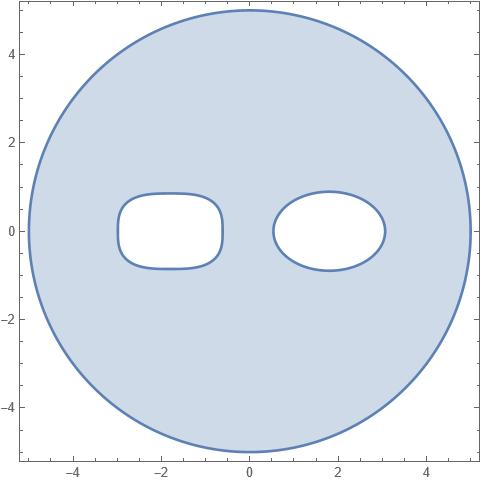
\includegraphics[width=0.75\textwidth]{pictures/14.jpeg}
\end{center}

%----------------------------------------
% 1. Физическая постановка задачи
%----------------------------------------
\section*{Физическая постановка задачи}

В данной задаче необходимо найти распределение электростатического потенциала в двумерной области, содержащей три электрода:

\begin{itemize}
    \item \textbf{Внешний электрод}, задающий граничные условия \( \varphi = 0 \) на окружности \( x^2 + y^2 = 25 \).
    \item \textbf{Электрод 1}, имеющий потенциал \( 7\,\text{В} \), описывается неявным уравнением \( (3|\tfrac{9}{5}+x|^3)/10 + (4|y|^3)/5 = 1/2 \).
    \item \textbf{Электрод 2}, имеющий потенциал \( -8\,\text{В} \), описывается уравнением \( |\tfrac{-9}{5} + x|^2/2 + |y|^2 = 4/5 \).
\end{itemize}

Внутри области потенциал удовлетворяет уравнению Лапласа:
\[
\nabla^2 \varphi = 0.
\]

Далее необходимо построить \textbf{силовую линию}, проходящую через точку \((0,\,-2)\). Силовые линии в электростатике определяются направлением вектора напряжённости поля \(\mathbf{E} = - \nabla \varphi\).

%----------------------------------------
% 2. Метод решения
%----------------------------------------
\section*{Метод решения}

\textbf{Решение уравнения Лапласа.} Численно используется метод Якоби на равномерной сетке \((241\times241)\) в квадрате \([-6,6]\times[-6,6]\). На узлах, соответствующих электродам, потенциал фиксирован в соответствии с граничными условиями (0\,В, 7\,В и -8\,В).

\textbf{Построение силовой линии.} Силовая линия определяется уравнением
\[
\frac{d\mathbf{r}}{ds} = \frac{-\nabla \varphi}{\|\nabla \varphi\|}.
\]

Интегрирование производится в двух направлениях от заданной точки, пока траектория не достигнет какого-либо электрода.

%----------------------------------------
% 3. Краткие фрагменты кода
%----------------------------------------
\section*{Краткие фрагменты кода}

Ниже приведены небольшие выдержки из кода для иллюстрации принципа работы.

\subsection*{Решение уравнения Лапласа (Jacobi)}
\begin{minted}[fontsize=\footnotesize, linenos]{python}
def solve_potential(x_min, x_max, y_min, y_max, nx, ny, tol_bound):
    x = np.linspace(x_min, x_max, nx)
    y = np.linspace(y_min, y_max, ny)
    X, Y = np.meshgrid(x, y)
    V = np.zeros((ny, nx))

    # Boundary conditions
    # ... (setting potentials for electrodes)

    # Jacobi iterations
    for it in range(5000):
        V_old = V.copy()
        # ...
        if np.max(np.abs(V - V_old)) < 1e-4:
            break
    return x, y, V
\end{minted}

\subsection*{Построение силовой линии}
\begin{minted}[fontsize=\footnotesize, linenos]{python}
def compute_field_line(x, y, V, start_point, tol_bound):
    dx, dy = compute_gradient(x, y, V)
    interp_dx = RegularGridInterpolator((y, x), dx)
    interp_dy = RegularGridInterpolator((y, x), dy)

    def integrate_direction(pt0, sign):
        # ...
        return length, path

    L_forward, path_forward = integrate_direction(start_point, +1)
    L_backward, path_backward = integrate_direction(start_point, -1)
    # ...
    return total_length, field_line_path
\end{minted}

%----------------------------------------
% 4. Результаты и примеры работы
%----------------------------------------
\section*{Результаты и примеры работы}

В результате программа вычисляет распределение потенциала в заданной области, строит карту потенциала, стрелки поля и отображает силовую линию, проходящую через точку \((0,\,-2)\).

\vspace{-1cm}
\begin{center}
    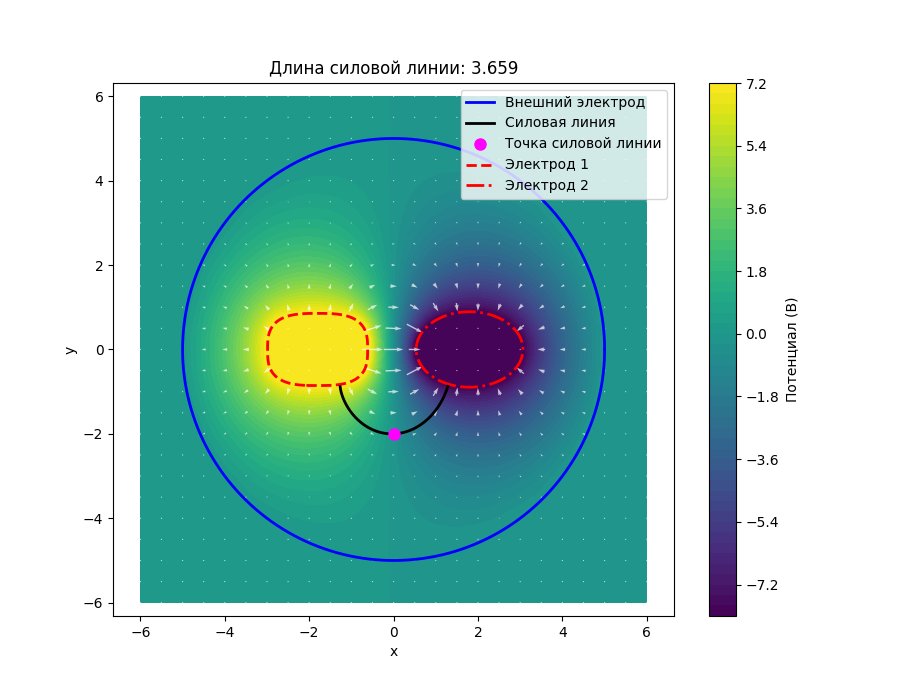
\includegraphics[width=0.75\textwidth]{pictures/result.png}
\end{center}

Скрипт сохраняет длину силовой линии в файл \texttt{IDZ1.txt}. Для варианта~14, длина силовой линии составила (примерно) 3.659 условных единиц.

%----------------------------------------
% 5. Выводы
%----------------------------------------
\section*{Выводы}

\begin{itemize}
    \item Метод Якоби позволяет решить уравнение Лапласа с заданными граничными условиями для электродов и найти потенциал в узлах сетки.
    \item По градиенту потенциала определяется электрическое поле \(\mathbf{E}\), а силовая линия --- это интегральная кривая, касательная к полю во всех точках.
    \item Численно проинтегрировав траекторию из заданной точки, удалось получить искомую силовую линию и вычислить её длину.
    \item Результаты визуализации наглядно показывают расположение электродов, распределение потенциала и направление силовой линии.
\end{itemize}

\end{document}
